% Compile with XeLaTeX (Overleaf: Menu -> Compiler -> XeLaTeX), run twice.
% XeLaTeX is needed only for the Vietnamese diacritics in the author names and in one quoted example.
\documentclass[conference]{IEEEtran}
\usepackage{iftex}
\ifPDFTeX
  \errmessage{Please compile this file with XeLaTeX (Overleaf: Menu -> Settings -> Compiler -> XeLaTeX)}
  \stop
\fi
\usepackage{fontspec}
\IfFontExistsTF{Times New Roman}{\setmainfont{Times New Roman}}{\setmainfont{TeX Gyre Termes}}
\usepackage{amsmath,amssymb}
\usepackage{booktabs}
\usepackage{algorithm}
\usepackage{algpseudocode}
\usepackage{pgfplots}
\pgfplotsset{compat=1.16}
\usepackage{cite}
\usepackage[hidelinks]{hyperref}
\usepackage{url}
\usepackage{balance}
\newcommand{\src}[1]{{\normalfont\footnotesize\emph{Source:}~\cite{data} {\scriptsize\texttt{#1}}}}
\newcommand{\RM}{results/recorded\_20261103\_234305}
\newcommand{\RS}{results/supplement\_20261104\_025037}

\begin{document}

\title{Byte-Oriented Pattern Matching for NLP Training-Data Filtering: An Empirical Study of Brute Force, KMP, k-KMP and Aho--Corasick}

\author{\IEEEauthorblockN{Đoàn Đăng Khoa (QE210117), Lâm Duy Phát (DE201087), Phạm Võ Ngọc Hân (QE210171),\\
Hoàng Quốc Tuấn (QE210261), Nguyễn Thị Minh Châu (QE210105)}
\IEEEauthorblockA{Group 2, CSD203 -- Data Structures and Algorithms with Python, Class AI21B, FPT University}}

\maketitle

\begin{abstract}
Keyword-based filtering of training corpora for language models must report every occurrence of up to thousands of keywords in large byte streams. We compare Brute Force (BF), Knuth--Morris--Pratt (KMP), multi-pattern KMP (k-KMP) and Aho--Corasick with failure and output links (AC), all implemented in pure Python over NFC-normalized UTF-8 bytes, against the C-level \texttt{bytes.find} baseline. Across 306 planned configurations on Vietnamese and English Wikipedia, random and adversarial corpora (287 completed, 19 timeouts, zero disagreements with a test oracle), scan time grows linearly with text size for both BF and KMP. On natural text both perform about one comparison per byte, yet KMP is 1.91--1.99$\times$ faster because of loop overhead in BF; a BF variant that tests the first byte before entering its inner loop is 1.75$\times$ faster than KMP. On an adversarial repeated-prefix corpus, KMP is 21.69$\times$ faster at pattern length 64. As the number of keywords grows from 1 to 1{,}000, AC scan time increases by only 50.4\%, whereas k-KMP grows roughly linearly and times out at 1{,}000 keywords. AC is 87.64$\times$ faster than k-KMP at 100 keywords and 4.14--4.27$\times$ faster than \texttt{bytes.find} called from a Python loop at 1{,}000 keywords on T1 and T2, at the cost of 14.02$\times$ more build memory. An ablation study shows that removing the failure link or the output link slows AC by 1.83$\times$ and 1.41$\times$, respectively, at 1{,}000 keywords, but not at a single keyword.
\end{abstract}

\begin{IEEEkeywords}
string matching, KMP, Aho--Corasick, ablation study, NLP data filtering
\end{IEEEkeywords}

\section{Introduction}
Before a large language model is trained, its corpus is commonly filtered against keyword lists~\cite{t5} in order to remove toxic content or personal information, or to assign topic labels. Such lists may contain thousands of keywords, while the text to be scanned often reaches tens of mebibytes or more. Classic algorithms such as Brute Force (BF) and Knuth--Morris--Pratt (KMP)~\cite{kmp} are designed for a single pattern, so running them once per keyword costs $O(k\cdot N)$ for $k$ patterns and a text of $N$ bytes. Aho--Corasick (AC)~\cite{ac} generalizes the KMP failure function to a trie that holds the whole pattern set and scans the text in a single pass in $O(N+Z)$ time, where $Z$ is the number of matches, independently of $k$.

The overall question of this study is: \emph{how can one to thousands of keywords be found completely and exactly in Vietnamese and English corpora with the highest throughput when the algorithms are implemented in pure Python?} We divide it into three research questions, each paired with a hypothesis (H) that is tested in Section~\ref{sec:results}:
\begin{itemize}
\item \textbf{RQ1 (scale):} How do the running time, throughput and number of byte comparisons of BF and KMP change as the text grows from 1 to 16~MiB? \emph{H1:} Both grow linearly in $N$; on natural text BF is as fast as or faster than KMP, because most alignments fail at the first byte.
\item \textbf{RQ2 (data conditions):} How do the alphabet size $\sigma$, the pattern length $m$ and repeated-prefix structure affect the gap between BF and KMP? \emph{H2:} A small $\sigma$ and repeated prefixes make BF slow down sharply with $m$, whereas KMP is independent of $m$.
\item \textbf{RQ3 (multiple patterns and ablation):} As the number of keywords $k$ grows from 1 to 1{,}000, how does AC compare with k-KMP in preprocessing time, scan time and memory, and how much do the failure link and the output link contribute? \emph{H3:} AC scan time is nearly independent of $k$, k-KMP grows linearly in $k$, and AC pays for this with memory.
\end{itemize}
Our contributions are a unified pure-Python implementation of all four algorithms over UTF-8 bytes together with a test oracle, a matrix of 306 configurations measured under a reproducible protocol, and an ablation study that isolates the roles of the failure link and the output link.

\section{Background and Related Work}
KMP~\cite{kmp} and Aho--Corasick~\cite{ac} are the foundational algorithms for single-pattern and multi-pattern exact matching, and the textbook by Goodrich et al.~\cite{goodrich} presents BF, KMP and tries in Python. Production corpus filters usually call libraries written in C; this study instead compares the algorithms when they are implemented in pure Python under one common data convention, and uses \texttt{bytes.find} only as a reference baseline. Skip-based single-pattern algorithms such as Boyer--Moore~\cite{bm} are outside the scope of this study.

\subsection{Brute Force and KMP}
BF tries every starting position $i$, compares $T[i+j]$ with $P[j]$, and stops at the first mismatching byte; its worst-case cost is $O(N\cdot m)$ with $O(1)$ extra memory. KMP~\cite{kmp} precomputes a table $\pi$, where $\pi[i]$ is the length of the longest proper prefix of $P[0..i]$ that is also a suffix of it. When a mismatch occurs after $j$ matched bytes, KMP sets $j\leftarrow\pi[j-1]$ and retries the same text byte, so the text pointer never moves backwards. Because each byte increases $j$ by at most one and each fallback decreases it by at least one, the total number of comparisons is at most $2N$. After a full match, KMP sets $j\leftarrow\pi[m-1]$ so that overlapping matches are not missed. Preprocessing takes $O(m)$ time and scanning takes $O(N+Z)$.

\subsection{k-KMP}
k-KMP stores $k$ tables $\pi$ and $k$ states. The outer loop reads each byte once, and the inner loop advances all $k$ KMP machines. With $L=\sum_j |P_j|$, preprocessing takes $O(L)$ time and scanning takes $O(k\cdot N+Z)$; reading the text only once does not remove the factor $k$.

\subsection{Aho--Corasick}
AC~\cite{ac} is defined by three functions. \emph{goto} gives the edges of a trie that contains every pattern, so patterns with a common prefix share a branch. \emph{fail}$(u)$ points to the state that represents the longest proper suffix of the string at $u$ that is still present in the trie; since a failure link always points to a shallower node, the links are built in breadth-first (BFS) order. \emph{output} reports the patterns that end at the current state together with the patterns that are suffixes of it; the output link (dictionary suffix link) points directly to the nearest terminal node on the failure chain. The number of states satisfies $Q\le L+1$. For each byte, the automaton follows failure links while no edge exists, takes the goto edge and then reports the outputs. The number of state transitions is at most $2N$, and the scan costs $O(N+Z)$ when an edge lookup in a Python dictionary takes expected $O(1)$ time. For a single pattern, the trie is a path and its failure links coincide with the KMP table $\pi$.

The full DFA variant~\cite{ac} precomputes a 256-column transition table for every state, so each byte requires exactly one lookup, at the cost of memory proportional to $Q\times 256$. Under the course rules~\cite{rules} for five-member groups, the team is exempt from implementing this variant; Section~\ref{sec:discussion} analyzes it only theoretically.

\section{Methods}
\subsection{Data and Output Convention}
Texts and keywords are normalized to Unicode NFC~\cite{uax15} and encoded as UTF-8~\cite{utf8}, and every algorithm operates on \texttt{bytes}. A match position is a zero-based byte offset; for example, in the Vietnamese phrase ``bác sĩ'' the pattern ``sĩ'' starts at byte 5, because ``á'' occupies two bytes. Every match, including overlapping ones, must be reported, and empty patterns are rejected. The pattern identifier \texttt{pid} is the index of the keyword in the input list after NFC normalization and removal of duplicates (the first occurrence is kept); the keyword files used in this study contain no duplicates, so \texttt{pid} equals the line index of the keyword. Results are summarized as a count and an order-independent checksum:
\begin{equation}
\mathrm{check}=\sum_{(pos,\,pid)}\big((pos+1)\cdot 1000003+pid\big)\bmod 2^{64}.
\end{equation}
All algorithms must produce the same \texttt{count} and \texttt{check} for the same configuration.

\subsection{KMP Implementation}
Algorithm~\ref{alg:kmp} shows the KMP table construction and scan; k-KMP keeps $k$ copies of the state $j$ and advances them within the same byte loop. BF uses two nested loops and stops at the first mismatching byte. Table~\ref{tab:cx} summarizes the complexity of all algorithms.

\begin{algorithm}[t]
\caption{KMP table construction and scan}
\label{alg:kmp}
\begin{algorithmic}[1]
\State $\pi[0]\gets 0$; $j\gets 0$
\For{$i\gets 1$ \textbf{to} $m-1$}
  \While{$j>0$ \textbf{and} $P[i]\ne P[j]$} \State $j\gets\pi[j-1]$ \EndWhile
  \If{$P[i]=P[j]$} \State $j\gets j+1$ \EndIf
  \State $\pi[i]\gets j$
\EndFor
\State $j\gets 0$
\For{$i\gets 0$ \textbf{to} $N-1$}
  \While{$j>0$ \textbf{and} $T[i]\ne P[j]$} \State $j\gets\pi[j-1]$ \EndWhile
  \If{$T[i]=P[j]$} \State $j\gets j+1$ \EndIf
  \If{$j=m$} \State report $(i-m+1,\ pid)$; $j\gets\pi[m-1]$ \EndIf
\EndFor
\end{algorithmic}
\end{algorithm}

\begin{table}[t]
\caption{Complexity of the Algorithms ($L=\sum_j|P_j|$, $Z$ = Number of Matches)}
\label{tab:cx}
\centering
\begin{tabular}{@{}llll@{}}
\toprule
Algorithm & Preprocessing & Scan & Extra memory \\
\midrule
BF & -- & $O(N\cdot m)$ & $O(1)$ \\
KMP & $O(m)$ & $O(N+Z)$ & $O(m)$ \\
k-KMP & $O(L)$ & $O(k\cdot N+Z)$ & $O(L)$ \\
AC (failure links) & $O(L)$ & $O(N+Z)$ & $O(Q)$ edges \\
AC (DFA) & $O(Q\cdot 256)$ & $O(N+Z)$ & $O(Q\cdot 256)$ \\
\bottomrule
\end{tabular}
\end{table}

\subsection{Aho--Corasick Implementation}
Each state is a Python object (declared with \texttt{\_\_slots\_\_}) that holds a dictionary of byte-labelled edges, a \texttt{fail} pointer, an \texttt{output\_link} pointer and the list of patterns ending at that state. Algorithm~\ref{alg:ac} summarizes the construction and the scan, and Table~\ref{tab:map} maps each mechanism to the corresponding function in the source code.

\begin{algorithm}[t]
\caption{AC link construction (BFS) and scan}
\label{alg:ac}
\begin{algorithmic}[1]
\For{each child $c$ of the root} \State $c.\mathit{fail}\gets$ root; enqueue $c$ in $\mathit{queue}$ \EndFor
\While{$\mathit{queue}$ is not empty}
  \State $u\gets \mathit{queue}.\mathrm{popleft}()$
  \For{each edge $(b, v)$ of $u$}
    \State $f\gets u.\mathit{fail}$
    \While{$f\ne\mathrm{None}$ \textbf{and} $b\notin f.\mathit{children}$} \State $f\gets f.\mathit{fail}$ \EndWhile
    \State $v.\mathit{fail}\gets f.\mathit{children}[b]$ if $f\ne\mathrm{None}$ else root
    \If{$v.\mathit{fail}$ is terminal}
      \State $v.\mathit{output\_link}\gets v.\mathit{fail}$
    \Else
      \State $v.\mathit{output\_link}\gets v.\mathit{fail}.\mathit{output\_link}$
    \EndIf
    \State enqueue $v$ in $\mathit{queue}$
  \EndFor
\EndWhile
\State $s\gets$ root
\For{$i\gets 0$ \textbf{to} $N-1$}
  \While{$s\ne$ root \textbf{and} $T[i]\notin s.\mathit{children}$} \State $s\gets s.\mathit{fail}$ \EndWhile
  \State $s\gets s.\mathit{children}.\mathrm{get}(T[i],\ \text{root})$
  \If{$s$ is terminal}
    \State $t\gets s$
  \Else
    \State $t\gets s.\mathit{output\_link}$
  \EndIf
  \While{$t\ne\mathrm{None}$}
    \State report $(i-|P|+1,\ pid)$ for each pattern $P$ at $t$
    \State $t\gets t.\mathit{output\_link}$
  \EndWhile
\EndFor
\end{algorithmic}
\end{algorithm}

\begin{table}[t]
\caption{Mapping of Mechanisms to \texttt{src/ac\_fail.py}}
\label{tab:map}
\centering
\begin{tabular}{@{}ll@{}}
\toprule
Mechanism & Function / attribute \\
\midrule
goto (byte trie) & \texttt{\_build\_trie}, \texttt{State.children} \\
Failure link (BFS) & \texttt{\_build\_failure\_and\_output\_links} \\
Output link & \texttt{State.output\_link} \\
Full scan & \texttt{scan\_hits}, \texttt{scan\_counted} \\
Ablation: no output link & \texttt{scan\_no\_output} \\
Ablation: no failure link & \texttt{scan\_no\_fail} \\
\bottomrule
\end{tabular}
\end{table}

\subsection{Ablation Design}
Following the common framework of the course~\cite{rules}, RQ3 disables one mechanism at a time. The variant without output links still uses failure links for state transitions, but after every byte it must walk the entire failure chain up to the root to find terminal nodes. The variant without failure links (which implies no output links) uses only the trie and restarts from the root at every byte position, with a worst-case cost of $O(N\cdot d)$, where $d$ is the depth of the trie. The three variants share the same construction step, so any difference comes from the scan alone, and their results must be identical.

\section{Experimental Setup}
\textbf{Machine.} Intel Core 7 240H (10 cores, 16 threads), 32~GiB RAM, Windows 11 build 26300, CPython 3.14.8, Balanced power plan, on AC power.

\textbf{Corpora.} T1 and T2 are Vietnamese and English Wikipedia~\cite{wiki} (configuration \texttt{20231101.vi/en}), NFC-normalized and cut to 1--16~MiB. T3 consists of uniformly random bytes over $\sigma\in\{2,4,26,256\}$ symbols. T4 is a text consisting only of the byte \texttt{a}, searched with the pattern $a^{m-1}b$, which is the worst case for BF.

\textbf{Matrix.} RQ1 uses T1 and T3 ($\sigma=26$) with $N\in\{1,2,4,8,16\}$~MiB and a 16-byte pattern. RQ2A uses T3 with $N=4$~MiB, $m=64$ and four values of $\sigma$. RQ2B uses T4 with $N=4$~MiB and $m\in\{8,64,1024\}$. RQ3 uses T1 and T2 at 4 and 16~MiB with $k\in\{1,10,100,1000\}$ and compares AC, k-KMP and \texttt{bytes.find}; the ablation runs on T1 and T2 at 4~MiB. In total there are 306 configurations. The three seeds 11, 29 and 47 vary the patterns and keyword sets; RQ2B is deterministic, so each value of $m$ is a single configuration without a seed, and its reported time is the median of the three timed repetitions.

\textbf{Protocol.} Every measurement runs in a fresh process, and data loading and normalization finish before the timed region. A timing run consists of one warm-up and three timed repetitions, and the median is taken per seed. Counting runs (comparisons, failure fallbacks, state transitions and output steps) and memory runs (\texttt{tracemalloc} around the construction step) are executed separately so that they do not affect the timings. Time is measured with \texttt{time.perf\_counter\_ns()}~\cite{pydoc} separately for construction and for the scan. The scan time includes the cost of the shared result collector, whose \texttt{hit()} callback updates the count and the checksum for every match; this cost is the same for all algorithms in a given configuration. The garbage collector remains enabled in every run (\texttt{gc.disable()} is never called), so natural collections are included in the measured time, and \texttt{PYTHONHASHSEED=0} keeps hash ordering stable. Each process is limited to 60~s through \texttt{subprocess.run(..., timeout=60)}; runs that exceed this limit are recorded as \texttt{timeout} and are never assigned a number. Throughput is computed as $(N/2^{20})/(t/1000)$~MiB/s. Unless stated otherwise, a speedup is the median of the per-seed ratios computed from unrounded times, so it may differ slightly from the ratio of the rounded medians shown in the tables. The main session took place on 3--4 November 2026 and was video-recorded; the supplementary session for RQ2A and the auxiliary BF experiment has its own CSV files. The project repository~\cite{repo} contains the source code (\texttt{src/}, \texttt{bench/}), the tests (\texttt{tests/}) and the raw measurements of both sessions in \texttt{results/}, including corpus and keyword hashes, per-seed minimum and maximum times, and the expected oracle results.

\section{Results and Discussion}
\label{sec:results}
\subsection{Correctness}
Of the 306 configurations, 287 completed and 19 timed out. A test oracle based on \texttt{bytes.find}, which restarts each search at $pos+1$ so that overlapping matches are kept and shares no code with the four algorithms under test, checked 1{,}374 rows of the main matrix and 120 rows of RQ2A and found no disagreement. The test suite consists of 68 passing tests (one skipped) and 10{,}000 fuzz cases (seed 11) that cover small alphabets, raw bytes, Unicode NFC/NFD input and prefix--suffix overlaps. The ablation variants produce identical results for every seed.

\subsection{RQ1: Text Size}
Fig.~\ref{fig:rq1} shows that the throughput of both algorithms stays nearly constant as $N$ grows: about 10~MiB/s for BF and about 19~MiB/s for KMP. When $N$ grows 16-fold, BF time rises from 100.4 to 1{,}617.7~ms and KMP time from 51.1 to 819.4~ms, i.e., by 16.11$\times$ and 16.05$\times$ (computed from unrounded medians), respectively, which is linear growth. T3 shows the same trend. \emph{Hypothesis check (H1):} the linear-growth part is confirmed, but the prediction about the speed of BF is rejected, as analyzed below.

\begin{figure}[t]
\centering
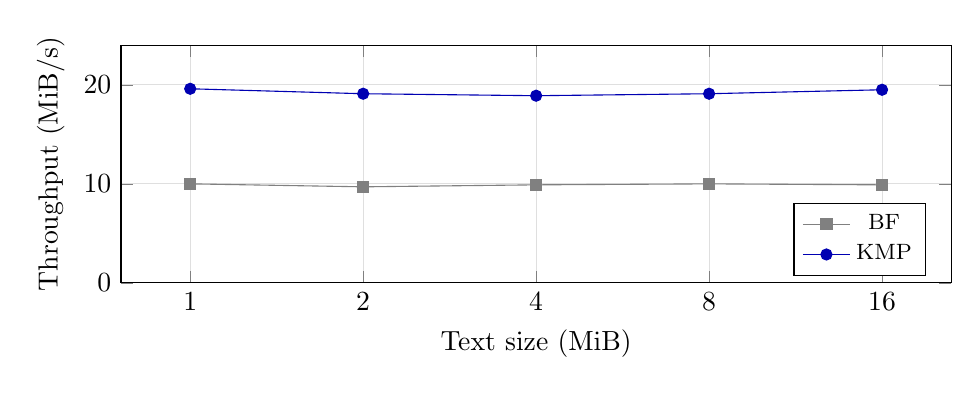
\begin{tikzpicture}
\begin{axis}[width=\columnwidth, height=4.6cm, xmode=log, log basis x=2,
  xtick={1,2,4,8,16}, xticklabels={1,2,4,8,16},
  xlabel={Text size (MiB)}, ylabel={Throughput (MiB/s)},
  ymin=0, ymax=24, legend pos=south east, legend style={font=\footnotesize},
  grid=major, grid style={gray!25}]
\addplot[mark=square*, gray] coordinates {(1,10.0) (2,9.7) (4,9.9) (8,10.0) (16,9.9)};
\addlegendentry{BF}
\addplot[mark=*, blue!70!black] coordinates {(1,19.6) (2,19.1) (4,18.9) (8,19.1) (16,19.5)};
\addlegendentry{KMP}
\end{axis}
\end{tikzpicture}
\caption{RQ1: throughput of BF and KMP on T1 with a 16-byte pattern, median of three seeds.\\ \src{\RM/analysis/summary.csv}}
\label{fig:rq1}
\end{figure}

Hypothesis H1 predicted that BF would be as fast as or faster than KMP on natural text, because most alignments fail at the first byte. The first part of this prediction holds: on T1 at 4~MiB, BF performs 1.050 and KMP 1.029 comparisons per byte. Nevertheless, KMP is 1.91--1.99$\times$ faster (211.1 versus 403.3~ms at 4~MiB). In CPython the cost lies in the number of bytecode instructions rather than in the comparisons themselves: at every position BF creates a new inner \texttt{range(m)} loop, even though the loop usually runs once and then breaks. A supplementary experiment on T3 at 4~MiB ($m=16$, three seeds) confirms this mechanism. The original BF takes 387.7~ms and KMP 200.1~ms, whereas a BF variant that tests the first byte before entering the inner loop takes only 114.5~ms, which is 1.75$\times$ faster than KMP. In isolation, the inner-loop structure costs 299.3~ms against 123.6~ms for a flat loop (2.42$\times$). This variant is used only as an explanation and does not replace the original BF in the RQ1 results.

\subsection{RQ2: Data Conditions}
Table~\ref{tab:rq2} summarizes both experiments. In RQ2A, the number of comparisons per byte made by BF matches the expected value $1+1/\sigma+1/\sigma^2+\dots=\sigma/(\sigma-1)$, because each subsequent byte is compared only if all preceding bytes matched, each with probability $1/\sigma$. BF time decreases as $\sigma$ grows. KMP is 1.72--2.10$\times$ faster than BF in terms of the ratio of medians, even at $\sigma=256$ where both perform almost the same number of comparisons; this is the same implementation overhead observed in RQ1.

\begin{table}[t]
\caption{RQ2: Scan Time (ms), $N=4$~MiB\\ \src{RQ2A: \RS/analysis/summary.csv}\\ \src{RQ2B: \RM/t4\_current.csv}}
\label{tab:rq2}
\centering
\setlength{\tabcolsep}{4pt}
\begin{tabular}{@{}rrrcc@{}}
\toprule
\multicolumn{5}{@{}l}{\textbf{RQ2A}: T3 random bytes, $m=64$, median of three seeds} \\
$\sigma$ & BF & KMP & BF comp./byte & $\sigma/(\sigma-1)$ \\
\midrule
2 & 567.0 & 326.6 & 2.000 & 2.000 \\
4 & 443.1 & 258.0 & 1.333 & 1.333 \\
26 & 409.0 & 210.8 & 1.040 & 1.040 \\
256 & 395.9 & 188.6 & 1.004 & 1.004 \\
\midrule
\multicolumn{5}{@{}l}{\textbf{RQ2B}: T4, $T=a^N$, $P=a^{m-1}b$, no seed (deterministic)} \\
$m$ & BF & KMP & BF comp. & KMP comp. \\
\midrule
8 & 1{,}380.9 & 420.3 & 33.6~M & 8.39~M \\
64 & 9{,}058.1 & 417.6 & 268.4~M & 8.39~M \\
1024 & timeout & 469.0 & -- & 8.39~M \\
\bottomrule
\end{tabular}
\end{table}

In RQ2B, BF matches $m-1$ bytes \texttt{a} before failing at every position, so it performs exactly $(N-m+1)\cdot m$ comparisons (33.6 million for $m=8$ and 268.4 million for $m=64$) and exceeds 60~s for $m=1024$. Since $\pi(a^{m-1}b)=[0,1,\dots,m-2,0]$, KMP falls back by one step and then matches immediately, so it always performs about $2N\approx 8.39$ million comparisons regardless of $m$. KMP is 21.69$\times$ faster at $m=64$. \emph{Hypothesis check (H2):} confirmed; the cost of BF follows $(N-m+1)\cdot m$ exactly, while the comparison count of KMP stays essentially constant in $m$.

\subsection{RQ3: Multiple Keywords}
Table~\ref{tab:rq3} and Fig.~\ref{fig:rq3} report the results on T1 at 4~MiB. The number of comparisons per byte made by k-KMP is approximately $k$ (1.06, 10.33 and 102.22), its time grows almost linearly in $k$, and it exceeds 60~s for all three seeds at $k=1{,}000$. AC stays at 1.06--1.33 comparisons per byte, and its time grows by only 50.4\% while $k$ grows 1{,}000-fold; the increase comes from additional failure fallbacks and from the number of matches $Z$, not from a factor of $k$. At $k=100$, AC is 87.64$\times$ faster than k-KMP (median of per-seed ratios). At $k=1$, AC and KMP both perform 1.06 comparisons per byte, consistent with the observation that the failure links of a single-pattern trie coincide with $\pi$. \emph{Hypothesis check (H3):} confirmed for both time and memory (see below).

\begin{table}[t]
\caption{RQ3: T1, 4~MiB, Median of Three Seeds (TO = Timeout at 60~s)\\ \src{\RM/analysis/summary.csv, build\_only.csv}}
\label{tab:rq3}
\centering
\setlength{\tabcolsep}{3.5pt}
\begin{tabular}{@{}lrrrr@{}}
\toprule
& $k=1$ & $k=10$ & $k=100$ & $k=1{,}000$ \\
\midrule
AC scan (ms) & 238.9 & 288.0 & 325.8 & 359.2 \\
k-KMP scan (ms) & 559.1 & 3{,}117.3 & 28{,}555.2 & TO \\
\texttt{bytes.find} (ms) & 1.2 & 13.6 & 143.1 & 1{,}530.7 \\
\midrule
AC comp./byte & 1.06 & 1.21 & 1.33 & 1.30 \\
k-KMP comp./byte & 1.06 & 10.33 & 102.22 & TO \\
\midrule
AC states $Q$ & 20 & 143 & 1{,}205 & 9{,}343 \\
AC build memory (KiB) & 6.4 & 49.2 & 464.5 & 3{,}747.2 \\
k-KMP memory (KiB) & 0.8 & 2.9 & 23.9 & 267.2 \\
AC build time (ms) & 0.0435 & 0.1372 & 2.9889 & 10.4823 \\
\bottomrule
\end{tabular}
\end{table}

The \texttt{bytes.find} baseline performs each search in C, but it is driven by a Python loop over the keywords, and every match is still reported through a Python \texttt{while} loop and a \texttt{hit()} call. It is the fastest method for $k\le 100$, but because it scans the text once per keyword, its time also grows with $k$. At $k=1{,}000$, AC is 4.21$\times$ faster than this baseline on T1 at 4~MiB (median of per-seed ratios; the ratio of the medians in Table~\ref{tab:rq3} is 4.26$\times$), and 4.14--4.27$\times$ faster across T1 and T2 at 4 and 16~MiB.

The price of AC is memory: the number of states reaches 9{,}343 and the memory allocated during construction reaches 3{,}747.2~KiB at $k=1{,}000$, which is 14.02$\times$ that of k-KMP, because every state is a Python object with its own dictionary. Construction takes at most 10.48~ms, about 2.9\% of the corresponding scan time, so the construction cost of AC is small compared with its scan.

\begin{figure}[t]
\centering
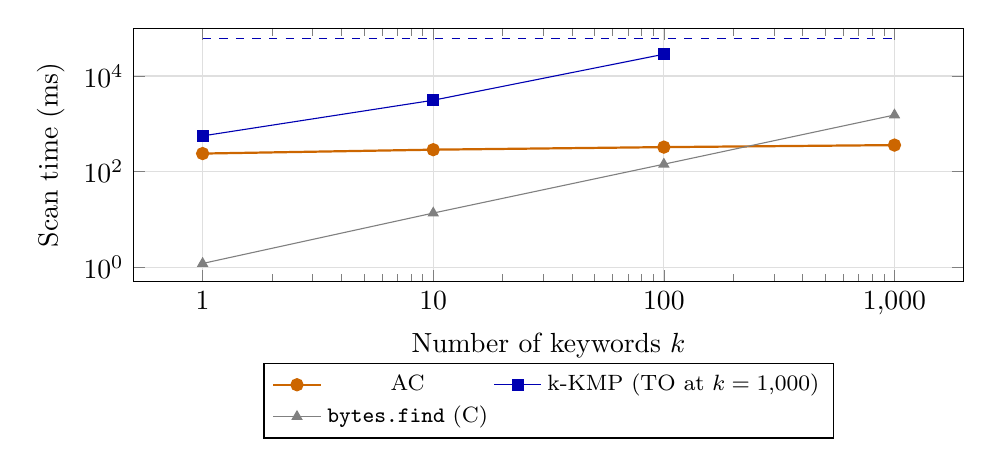
\begin{tikzpicture}
\begin{axis}[width=\columnwidth, height=4.8cm, xmode=log, ymode=log,
  xtick={1,10,100,1000}, xticklabels={1,10,100,{1,000}},
  xlabel={Number of keywords $k$}, ylabel={Scan time (ms)},
  ymin=0.5, ymax=100000, legend style={font=\footnotesize, at={(0.5,-0.32)}, anchor=north, legend columns=2},
  grid=major, grid style={gray!25}]
\addplot[mark=*, orange!80!black, thick] coordinates {(1,238.9) (10,288.0) (100,325.8) (1000,359.2)};
\addlegendentry{AC}
\addplot[mark=square*, blue!70!black] coordinates {(1,559.1) (10,3117.3) (100,28555.2)};
\addlegendentry{k-KMP (TO at $k=1{,}000$)}
\addplot[mark=triangle*, gray] coordinates {(1,1.2) (10,13.6) (100,143.1) (1000,1530.7)};
\addlegendentry{\texttt{bytes.find} (C)}
\addplot[blue!70!black, dashed, no markers, domain=1:1000, samples=2, forget plot] {60000};
\end{axis}
\end{tikzpicture}
\caption{RQ3: scan time versus $k$ on T1 at 4~MiB (log--log scale). The dashed line marks the 60~s limit.\\ \src{\RM/analysis/summary.csv}}
\label{fig:rq3}
\end{figure}

\subsection{Aho--Corasick Ablation}
Table~\ref{tab:abl} compares the three variants. The ablation configurations are separate cells of the matrix and were measured in separate runs, so the times of the full version differ slightly from the AC row of Table~\ref{tab:rq3} (for example, 245.5 versus 238.9~ms at $k=1$); comparisons are therefore made only within each table. At $k=1{,}000$, disabling the failure link raises the comparison count from 1.30 to 2.36 per byte and slows AC by 1.83$\times$ (median of per-seed ratios), because the scan has to restart from the root at every position. Disabling the output link slows AC by 1.41$\times$: the full version needs only 1{,}807 output-link jumps to report all matches, whereas the variant without output links visits about 5.7 million nodes on failure chains (medians over the three seeds). These two counters measure different kinds of work and are not CPU cycle counts. At small scale the relationship is reversed: at $k=1$, the variant without failure links is 11\% faster, because the trie is very shallow and natural text almost always mismatches at the root; from $k=10$ onwards, the full version is already slightly faster, and the gap widens as $k$ grows.

\begin{table}[t]
\caption{Ablation: Scan Time (ms), T1, 4~MiB, Median of Three Seeds\\ \src{\RM/analysis/summary.csv}}
\label{tab:abl}
\centering
\setlength{\tabcolsep}{4pt}
\begin{tabular}{@{}lrrrr@{}}
\toprule
Variant & $k=1$ & $k=10$ & $k=100$ & $k=1{,}000$ \\
\midrule
Full & 245.5 & 297.7 & 340.3 & 359.8 \\
No output link & 228.2 & 308.4 & 399.0 & 506.4 \\
No failure link & 218.2 & 309.5 & 454.7 & 655.8 \\
\bottomrule
\end{tabular}
\end{table}

\subsection{Discussion}
\label{sec:discussion}
\textbf{BF and KMP on natural text.} The measurements confirm the mechanism stated in H1: BF almost always fails at the first byte, so the theoretical advantage of KMP in comparison count disappears. The timing result, however, contradicts the prediction (KMP is 1.9$\times$ faster), and the supplementary experiment shows that the cause lies in the loop structure of the BF implementation rather than in the algorithm: once the inner loop is skipped at most positions, BF becomes faster than KMP. In CPython, the speed ranking of two algorithms of the same order depends on implementation constants.

\textbf{Failure links versus DFA.} The failure-link version stores sparse edges in dictionaries, so its memory is proportional to the number of actual edges ($Q-1$), but a byte may trigger several failure fallbacks. A DFA precomputes the transition for every byte value, removing the fallback loop and requiring exactly one table lookup per byte, but it needs $Q\times 256$ cells; with $Q=9{,}343$ at $k=1{,}000$ this amounts to about 2.39 million cells, compared with 9{,}342 trie edges. Because the team did not implement the DFA, this statement is a model-based analysis rather than a measured result, and a ``cell'' does not correspond to an actual number of bytes in Python.

\textbf{Results beyond Big-O predictions.} Three observations stand out: (i) KMP is faster than BF despite an equal number of comparisons; (ii) AC in Python beats the \texttt{bytes.find} baseline, whose searches run in C, at $k=1{,}000$; and (iii) at $k=1$ the optimizations of AC bring no benefit. Together they show that a better asymptotic complexity wins only when the problem is large enough to offset the constant factors of the interpreter.

\section{Threats to Validity}
\emph{Measurement environment.} Because the garbage collector is enabled by default, a collection may fall inside a timed run; Windows is not a real-time operating system, and its scheduler may preempt the process. Taking medians, checking the CPU/wall-time ratio and re-running contended measurements reduce but do not eliminate this noise. Since the algorithms are implemented in pure Python, the timings reflect interpreter overhead; constants and speed rankings may differ in a compiled language.

\emph{Statistics and data.} All figures except RQ2B come from three seeds on a single machine with a single CPython version; because of the page limit, the tables report medians only; the per-seed minimum and maximum times are published in the summary files of the repository, and no confidence intervals or statistical tests are computed. The T1 and T2 corpora are nested prefixes, so increasing $N$ also adds new content, and increasing $k$ also changes the total pattern length and the match density. The three T3 files with $\sigma=2,4,256$ were generated with the same seed (42), so the three seeds vary only the patterns; the $\sigma=256$ file consists of raw bytes. The two measurement sessions took place at different times and under different background loads. Memory measured with \texttt{tracemalloc} covers only Python allocations during construction, not the resident set size (RSS). The 19 timeouts refer to the whole process. The test oracle is independent of the four algorithms under test, but it uses \texttt{bytes.find}, as does the library baseline, so it does not validate that baseline independently. The 26.47\% of T1 lines flagged at $k=1{,}000$ is neither a precision nor a recall figure, because no independent labels exist; the experiment evaluates pattern matching and processing cost, not the quality of content moderation. All conclusions are tied to the stated implementation, inputs and machine and do not imply a general advantage of Python over C.

\balance
\section{Conclusion}
In pure CPython, BF and KMP both scan in linear time; on natural text they perform almost the same number of comparisons, and their speed ranking depends on how the loops are implemented. KMP shows a clear advantage when the data contains repeated prefixes (21.69$\times$ at $m=64$) or a small alphabet. With many keywords, Aho--Corasick is nearly independent of $k$: it is 87.64$\times$ faster than k-KMP at 100 keywords and 4.14--4.27$\times$ faster than \texttt{bytes.find} called from a Python loop at 1{,}000 keywords on T1 and T2, in exchange for 14.02$\times$ more construction memory. Our conditional recommendations are as follows: use KMP for a single pattern; use Aho--Corasick for multiple patterns in pure Python; and, when a C library is allowed, use \texttt{bytes.find} for $k\le 100$ and Aho--Corasick for $k$ around 1{,}000. These recommendations apply only to the values of $k$ and the implementations that were tested.

\section*{Acknowledgment}
\textbf{AI usage statement.} The team used AI tools (Claude by Anthropic and Codex by OpenAI) to assist with merging and reviewing code, running tests, generating figures from CSV files and drafting the text of this report. Every number was taken from recorded measurement runs whose CSV files, including data hashes, are published in the project repository. The team members performed the final testing, verified the sources and take responsibility for the submitted content; AI tools did not replace the individual oral examination.

\begin{thebibliography}{5}
\bibitem{t5} C.~Raffel \emph{et al.}, ``Exploring the limits of transfer learning with a unified text-to-text transformer,'' \emph{J. Mach. Learn. Res.}, vol.~21, no.~140, pp.~1--67, 2020.
\bibitem{kmp} D.~E. Knuth, J.~H. Morris, and V.~R. Pratt, ``Fast pattern matching in strings,'' \emph{SIAM J. Comput.}, vol.~6, no.~2, pp.~323--350, 1977.
\bibitem{ac} A.~V. Aho and M.~J. Corasick, ``Efficient string matching: An aid to bibliographic search,'' \emph{Commun. ACM}, vol.~18, no.~6, pp.~333--340, 1975.
\bibitem{goodrich} M.~T. Goodrich, R.~Tamassia, and M.~H. Goldwasser, \emph{Data Structures and Algorithms in Python}. Hoboken, NJ, USA: Wiley, 2013, ch.~13.
\bibitem{bm} R.~S. Boyer and J.~S. Moore, ``A fast string searching algorithm,'' \emph{Commun. ACM}, vol.~20, no.~10, pp.~762--772, 1977.
\bibitem{rules} CSD203, ``General rules for group projects,'' class AI21B, Fall 2026, FPT University, Oct. 14, 2026. [Online]. Available in~\cite{repo}: \nolinkurl{docs/quy-dinh-chung-do-an-nhom-csd203.md}
\bibitem{uax15} M.~Davis and K.~Whistler, ``Unicode normalization forms,'' Unicode Standard Annex \#15, Unicode Consortium. Accessed: Nov. 16, 2026. [Online]. Available: \url{https://unicode.org/reports/tr15/}
\bibitem{utf8} F.~Yergeau, ``UTF-8, a transformation format of ISO 10646,'' RFC 3629, IETF, Nov. 2003.
\bibitem{wiki} Wikimedia Foundation, ``wikimedia/wikipedia,'' Hugging Face Datasets. Accessed: Nov. 15, 2026. [Online]. Available: \url{https://huggingface.co/datasets/wikimedia/wikipedia}
\bibitem{pydoc} Python Software Foundation, ``The Python standard library: \texttt{time}, \texttt{tracemalloc},'' Python 3.14 documentation. Accessed: Nov. 16, 2026. [Online]. Available: \url{https://docs.python.org/3.14/library/}
\bibitem{repo} Group 2, ``\texttt{Group-2-{}-{}-Pattern-Matching},'' GitHub repository, branch \texttt{main}, source code at commit \texttt{282a566}. Accessed: Nov. 16, 2026. [Online]. Available: \url{https://github.com/kittyhan124-glitch/Group-2---Pattern-Matching}
\bibitem{data} Group 2, ``Measured results of the pattern-matching benchmark (CSV),'' GitHub repository \texttt{Group-2-{}-{}-Pattern-Matching}, branch \texttt{main}, files \texttt{results/recorded\_20261103\_234305/*.csv} and \texttt{results/supplement\_20261104\_025037/*.csv}, commit \texttt{282a566}, the same commit as~\cite{repo} (the files are unchanged since they were added in \texttt{d09c685}). Accessed: Nov. 16, 2026. [Online]. Available: \url{https://github.com/kittyhan124-glitch/Group-2---Pattern-Matching/tree/main/results}
\end{thebibliography}

\end{document}
